\chapter{Estado del arte}

\section{BRDF Cook-Torrance}
Es un modelo anal\'itico permite representar con gran realismo materiales electricos y dielectricos con diferentes
grados de rugosidad y, en general, funciona bien para modelar cambios en el color que dependen del punto de vista.\\
Este modelo permite estudiar por separado las dos componentes de la luz, especular y difuso:

\begin{eqfloat}[!htb]
    \begin{equation}
        f_r = k_{d}f_{lambert} + k_sf_{cook-torrance}
    \end{equation}
    \caption{BRDF como suma de la componente difusa y especular}
\end{eqfloat}

siendo $k_d$ y $k_s$, parametros de peso que cumplen $k_d + k_s = 1$
\singlespacing
x
T\'ipicamente la componente difusa, utiliza el modelo de Lambert, que asume una distribuci\'on completamente uniforme a lo
largo de la superficie:\\

\begin{equation}
f_{Lambert} = \frac{diffuse}{\pi}
\end{equation}
\singlespacing

La componente especular es una funci\'on compuesta de otras tres funciones y un factor de normalizaci\'on en el
denominador.\\

\begin{equation}
    f(l, v) = \frac{F(w_i, h) G(w_i, h, w_o) D(h)} {4(n\cdot{w_i}) (n \cdot{w_o})}
\end{equation}
\singlespacing

    \subsection{T\'erminos del BRDF especular}
        El BRDF de Cook-Torrance est\'a compuesto por otras tres funciones y un factor de normalizaci\'on en el denominador.
        Las funciones D, F y G, se corresponden con la funci\'on de distribuci\'on de las normales, la ecuaci\'on de Fresnel,
        y la funci\'on de geometr\'ia.\\

        $D(l, v, h)$  es la funci\'on de distribuci\'on de las normales y se encarga de representar la rugosidad de una superficie
        y es el t\'ermino que afecta en mayor grado a la forma y taman\~no del brillo especular. T\'ipicamente el par\'ametro
        \textit{roughness} se utiliza para representar la cantidad de microfacetas alineadas con la normal h, cuanta mayor sea la
        la cantidad de de microfacetas alineadas, m\'as lisa parecer\'a la superficie.

        $$
        D(h) = \frac{\alpha^2}{\pi((n\cdot{h})^2(\alpha^2 - 1) + 1)^2}
        $$

        \begin{figure}[H]
            \vspace{0.5cm}
            \centering
            \frame{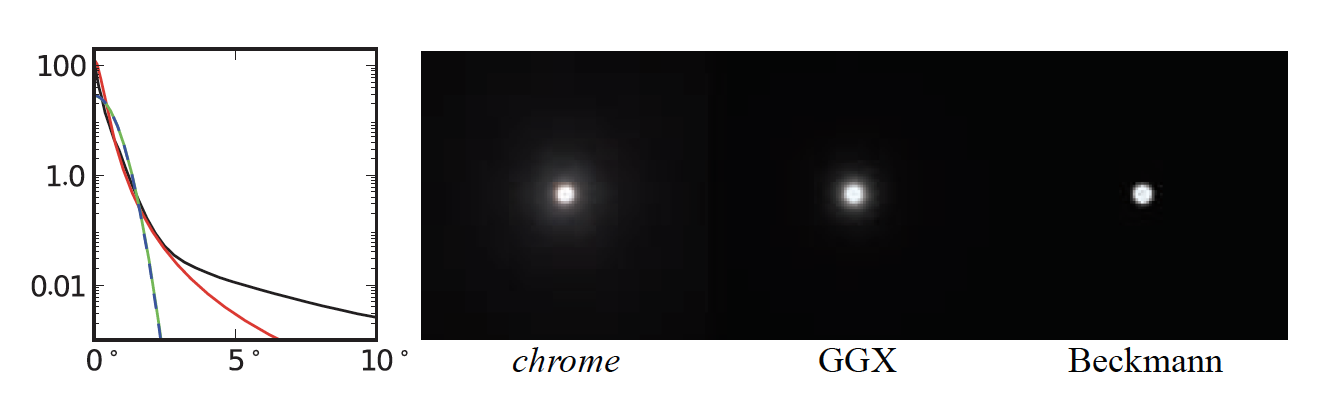
\includegraphics[scale=0.65]{ndf}}
            \caption{Representaci\'on gr\'afica de la funci\'on de geometr\'ia}
        \end{figure}

        $G(w_o)$ es la funci\'on de geometr\'ia. Esta funci\'on tiene en cuenta las oclusiones debidas a la propia superficie.
        Mientras que el t\'ermino de distribucion de las normales, $D(h)$, define la concentraci\'on de microfacetas con una normal h,
        no define si esas microfacetas son visible o no. El t\'ermino de geometr\'ia tiene en cuenta las dos cosas, la sombra
        y el enmascaramiento. La sombra representa que una microfaceta no es visible desde la direcci\'on de la luz, mientras que el
        enmascaramiento significa que una microfaceta no es visible desde la direcci\'on de vista y, por tanto, no contribuyen
        a la reflexi\'on.

        $$
        G(w_i, w_o) = G(w_i)G(w_o)
        $$
        \singlespacing
        $$
        G(w_o) = \frac{n\cdot{w_o}}{(n\cdot) (1 - k) + k}
        $$
        \singlespacing
        $$
        G(w_i) = \frac{n\cdot{w_i}}{(n\cdot) (1 - k) + k}
        $$
        \singlespacing

        \begin{equation}
        k = \frac{(roughness + 1)^2}{8}
        \end{equation}

        \begin{figure}[H]
            \vspace{0.5cm}
            \centering
            \frame{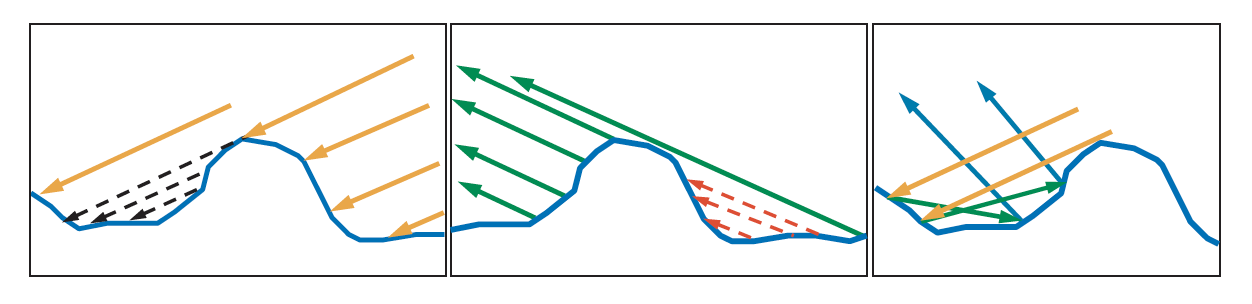
\includegraphics[scale=0.65]{microgeometria}}
            \caption{Representaci\'on gr\'afica de la sombra y el enmascaramiento en la funci\'on de geometr\'ia}
        \end{figure}

        $F(l, v, h)$ es la funci\'on de Fresnel. Representa la radiancia reflejada por un material seg\'un el \'angulo de incidencia
        de la luz. Para la mayor\'ia de los materiales no met\'alicos, las reflexiones son m\'as intensas bajo cuando el \'angulo
        de incidencia es muy agudo. En la mayor\'ia de los algoritmos de sombreado, el fresnel se utiliza a nivel de la macrosuperficie,
        sin embargo, al aplicar el fresnel sobre la normal de la microfacetas, se consigue un mayor grado de realismo para los valores
        altos de \textit{roughness}.

        $$
        F_{Schlick}(F_o, w_i, h) = F_o + (1 - F_o) (1 - (l\cdot{h}))^5
        $$

        \begin{figure}[H]
            \vspace{0.5cm}
            \centering
            \frame{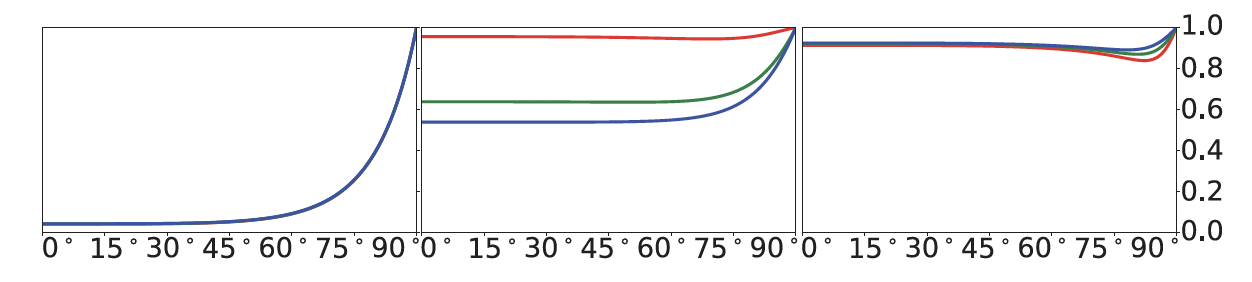
\includegraphics[scale=0.65]{fresnel}}
            \caption{Representaci\'on gr\'afica de la funci\'on de geometr\'ia}
        \end{figure}
        \singlespacing

        El denominador es una caracter\'istica t\'ipica de los modelos de microfacetas y es un factor de correci\'on debido al cambio
        de espacio entre el espacio local de las microfacetas y el espacio local de la macrosuperficie. Para modelos que no
        incluyen este factor, se puede aplicar un factor de sombreado directamente multiplicando el t\'ermino de geometr\'ia por

        \begin{equation}
        \frac{1}{4(n\cdot{l}) (n\cdot{v})}
        \end{equation}
        \singlespacing

        % La funci\on de distribuci\'on de las normales, aproxima la cantidad de microfacetas aproxima la alineadas con el
        % vector h, el medio entre el rayo de luz y el punto del vista. El par\'ametro que modela la rugosidad de una superficie
        % afecta en gran medida al resultado. Este es el factor m\'as caracter\'istico del modelo de microfacetas.
        % La funci\'on de geometr\'ia describe la cantidad de rayos ocluidos por las propias microfacetas.\\

        % Finalmente, la ecuaci\'on de fresnel describe el ratio de reflexi\'on de una superficie bajo diferentes \'angulos de
        % incidencia.\\

% \section{T\'erminos del BRDF}
% \todo[inline]{
%     Blinn \autocite{blinn77}, Beckmann \autocite{beckmann}, Walter \autocite{ggx}, Neumann \autocite{neumann}, Kelemen
%     \autocite{kelemen}, Smith \autocite{smith}, Karis \autocite{unreal}, \autocite{reed}
% }

\section{Disney Principled BRDF}
% \todo[inline]{Modelo emp\'irico basado en las observaciones de la tabla MERL}

\begin{figure}[H]
    \vspace{0.5cm}
    \centering
    \frame{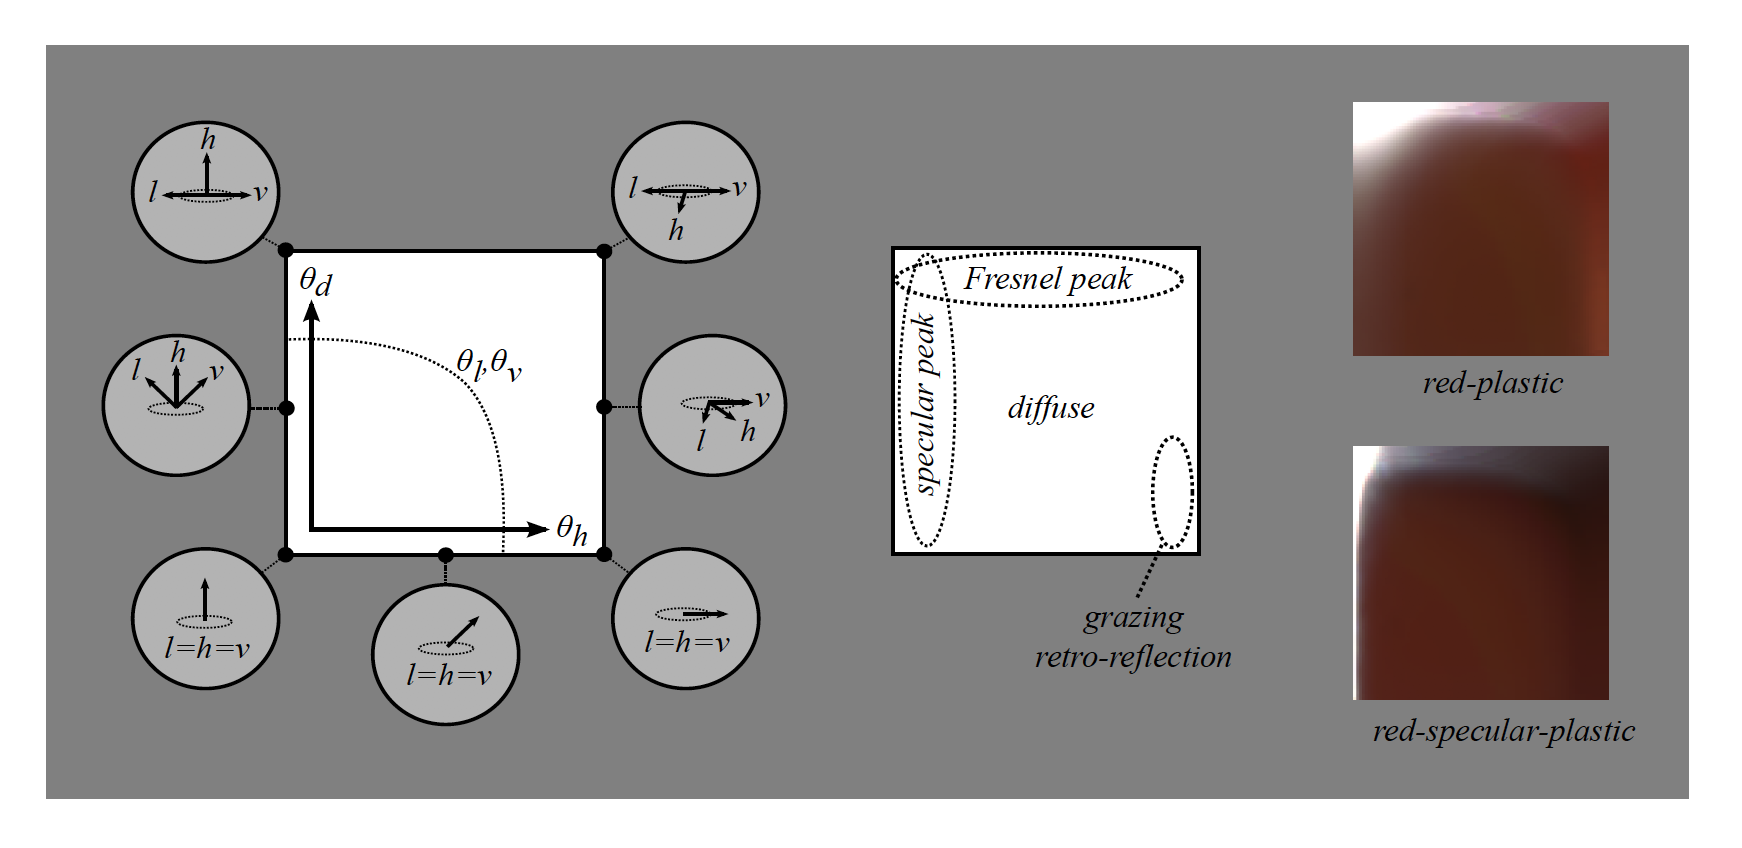
\includegraphics[scale=0.47]{slicespace}}
    \caption{Muestras de materiales MERL, junto a un esquema explicativo de las im\'agenes muestreadas}
    \vspace{0.5cm}
\end{figure}

El BRDF de Disney fue presentado por Brent Burley en 2012 y es el utilizado por Disney en sus peliculas de animacion. Es,
junto al modelo de Cook-Torrance, el mas utilizado en los motores de tiempo real, sin embargo, el modelo de Burley, es mas
amigable para los artistas, a costa de no ser completamente basado en fisica. Los parametros tienen nombres y valores que
definen que el aspecto de los materiales son mas intuitivos. Los lobulos adicionales, a diferencia del modelo de Cook-Torrance,
pueden variar mucho en forma y tamanho, por lo que es un modelo muy flexible, que permite representar con gran realismo una
amplia variedad de materiales.\\

Es conocido como \textit{principled} por cumplir una serie de m\'aximas, que se respetan en el modelo por encima de las leyes fisicas.
El modelo ha de ser intuitivo y no utilizar parametros que se refieran al modelo basado en fisica, debe tener el menor
numero de parametros posible, deben de estar normalizados, algunos valores pueden exceder su rango para permitir mayor
expresividad y, finalmente, todas las combinaciones de parametros deben de ser robustas y plausibles. Para ello utiliza los
par\'ametros: \textit{baseColor}, \textit{subsurface}, \textit{metal}, \textit{specular}, \textit{specularTint}, \textit{roughness},
\textit{sheen}, \textit{sheenTint}, \textit{clearCoat}, \textit{clearcoatGloss}

\begin{figure}[H]
    \vspace{0.5cm}
    \centering
      \frame{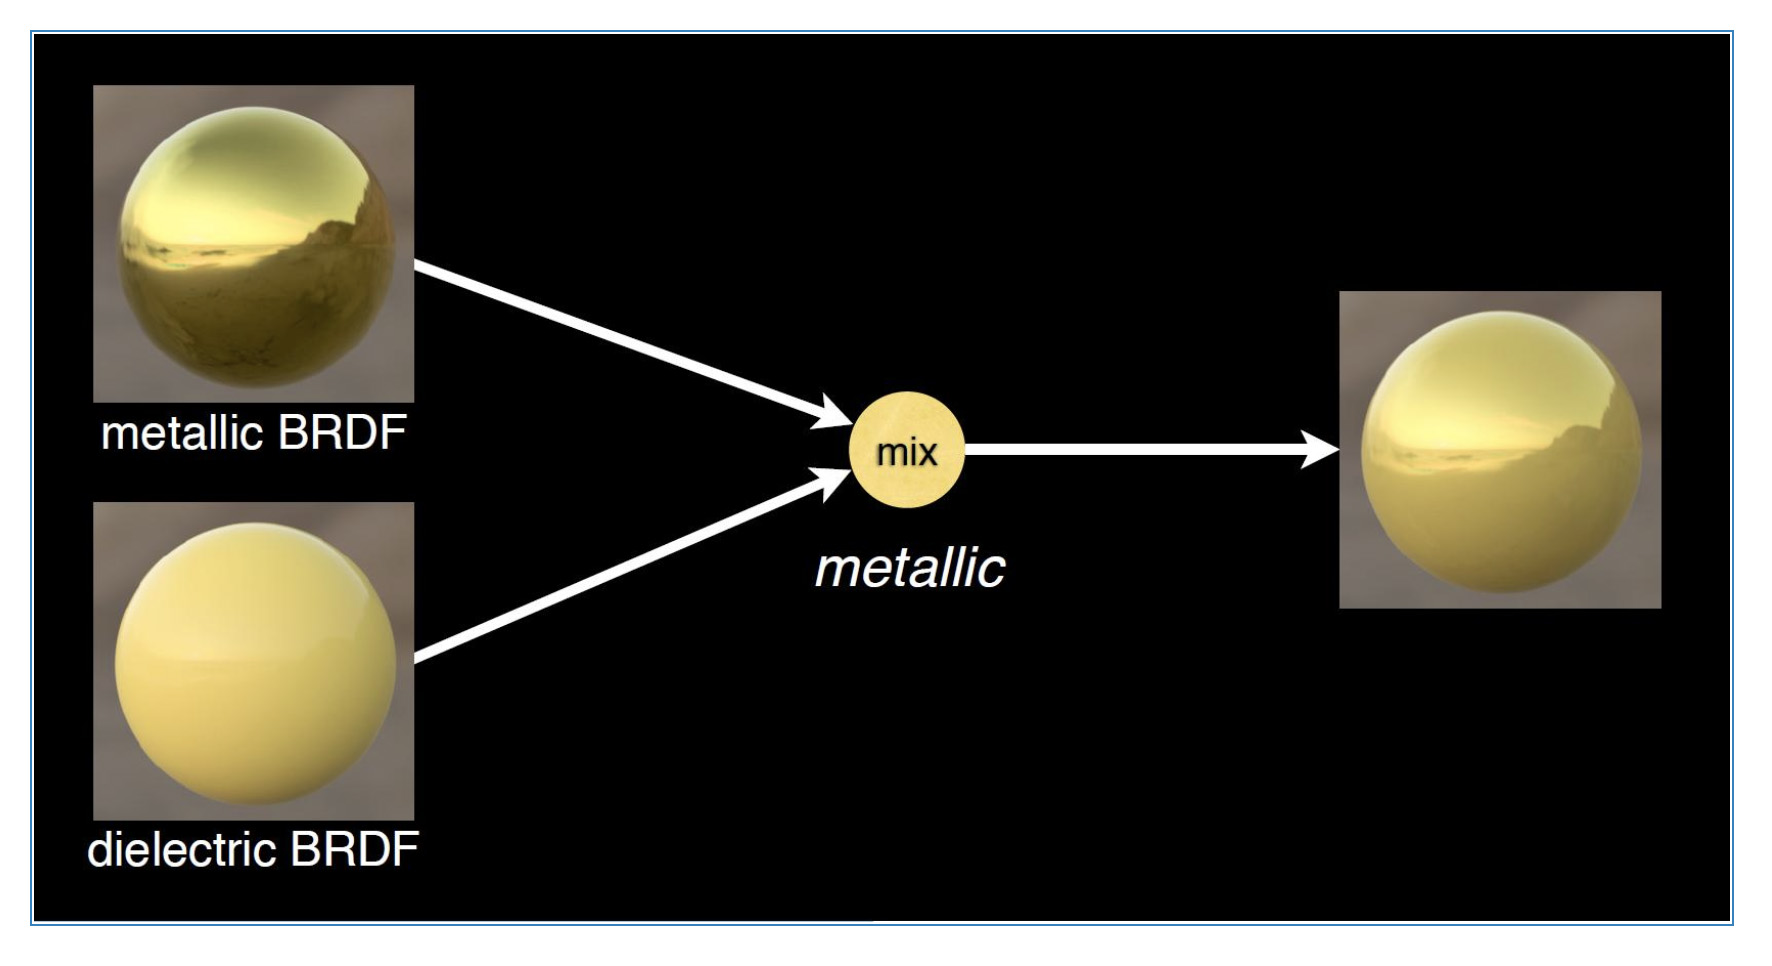
\includegraphics[scale=0.47]{disney}}
    \caption{Modelo de Disney}
\end{figure}
% \begin{itemize}
% 	\item \textit{baseColor}: el color de la superficie, comunmente utiliza un mapa.
% 	\item \textit{subsurface}: aproximacion para controlar el color de la reflexion difusa.
% 	\item \textit{metal}: interpolaci\'on lineal entre los dos modelos. El met\'alico no tiene
%     componente de reflexi\'on difusa y su componente de reflexi\'on especular es del mismo color que el color base. 
%     \item \textit{specular}: cantidad de luz incidente reflejada, se utiliza para controlar de forma intuitiva el \'indice de refracci\'on de
%     una superficie.
% 	\item \textit{specularTint}: par\'ametro que permite a los artistas controlar el color de la reflexi\'on especular sobre el color
% 	base.
% 	\item \textit{roughness}: describe la rugosidad de una superficie, afectando a la reflexi\'on difusa y especular.
% 	\item \textit{sheen}: permite mayor grado de control sobre la reflexi\'on especular, muy \'util sobre tejidos.
% 	\item \textit{sheenTint}: color del \textit{sheen}
% 	\item \textit{clearCoat}: un l\'obulo extra.
% 	\item \textit{clearcoatGloss}: permite controlar la rugosidad de este l\'obulo.
% \end{itemize}
    
    \subsection{Componente difusa}

    En base a las observaciones sobre los datos de MERL, el modelo difuso parece muy oscuro hacia los bordes, y aplicando
    la funci\'on de Fresnel, para intentar conseguir un modelo f\'isicamente plausible, parece oscurecer m\'as los bordes,
    acentuando el problema. Disney desarroll\'o un modelo emp\'irico, que utiliza la aproximaci\'on de Fresnel Schlick:

    \begin{equation}
        (1 - F(\theta_l) (1 - F(\theta_d)))
    \end{equation}
    \singlespacing


    Modific\'andolo para conseguir que la retrodispersi\'on dependa del valor de \textit{roughness} y as\'i
    adaptarse mejor a los datos obtenidos de MERL.

    \begin{equation}
    f_d = \frac{baseColor}{\pi}
    \left(  1 + (F_{D90} - 1)(1 - cos\theta_{wi})^5  \right)
    \left(  1 + (F_{D90} - 1)(1 - cos\theta_{wo})^5  \right)
    \end{equation}
    
    $$
    F_{D90} = 0.5 + 2roughness\cdot{cos^2\theta_d}
    $$

    \subsection{Componente especular}
        \subsubsection{F, t\'ermino de Fresnel}
            Para el especular, la aproximaci\'on de Fresnel Schlick es lo suficientemente precisa y mucho menos costosa que
            que la ecuaci\'on completa de Fresnel.

            \begin{equation}
            (1 - F(\theta_l) (1 - F(\theta_d)))^5
            \end{equation}

            $F_0$ representa la reflectancia de una incidencia del mismo \'angulo que la normal. $\theta_d$ es el \'angulo
            entre el vector $h$, y el de vista $w_o$. Es acrom\'actico para los diel\'ectricos y crom\'atico para los metales.

        \subsubsection{G, t\'ermino de geometr\'ia}
            En el t\'ermino G, Disney utiliza dos modelos diferentes, uno para el l\'obulo primario y otro para el de clearcoat.
            Para el l\'obulo primario, utiliza el modelo de Smith GGX, remapeando el valor de \textit{roughness} para evitar
            ganar demasiada energ\'ia hacia los bordes de materiales brillantes.

            $$
            G(l, v, h) = G_{GGX}(l)G_{GGX}(v)
            $$

            $$
            G_{GGX}(v) = \frac
            {2 (n \cdot{v})}
            {(n \cdot{v}) + \sqrt{ \alpha^2 + (1 - \alpha)^2 (n \cdot{v})^2 }}
            $$

            \begin{equation}
            \alpha = (0.5 + roughness / 2)^2
            \end{equation}
            \singlespacing

            Para el l\'obulo secundario se utiliza un valor fijo de $\alpha = 0.25$.

        \subsubsection{D, t\'ermino de distribuci\'on de las normales}
            La distribuci\'on GGX es equivalente a la de Trowbridge-Reitz, no tiene una cola lo suficientemente larga para la
            mayor\'ia de materiales.

            \begin{equation}
                D_{TR} = \frac
                {c}
                {(\alpha^2 cos^2 \theta_h + sin^2 \theta_h)^2}
            \end{equation}
            \singlespacing

            El modelo de Disney utiliza un exponente en el denominador que permite mayor control sobre el radio de la reflexi\'on
            especular, llamando a \'este t\'ermino Generalized Trowbridge-Reitz, o GTR:

            \begin{equation}
                D_{GTR} = \frac
                {c}
                {(\alpha^2 cos^2 \theta_h + sin^2 \theta_h)^\gamma}
            \end{equation}
            \singlespacing

            \todo[inline]{NDFs anisotr\'opicas}

            Los dos l\'obulos, primario y secundario utilizan la distribuci\'on GTR. El l\'obulo primario,
            que representa la reflexi\'on del material base, utiliza $\gamma = 2$ y puede ser diel\'etrico o met\'alico,
            isotr\'opico o anisotr\'opico. Por otra parte, el l\'obulo secundario representa la capa de \textit{clearcoat}
            sobre el material base, utiliza $\gamma = 1$ y suele ser isotr\'opico y no met\'alico.




\section{Iluminaci\'on indirecta en tiempo real}

Para los efectos de iluminacion global, se necesita conocer la irradiancia proviniente en todas
direcciones $w_i$ sobre la esfera $\Omega$.\\

\begin{figure}[H]
    \vspace{0.5cm}
    \centering
      \frame{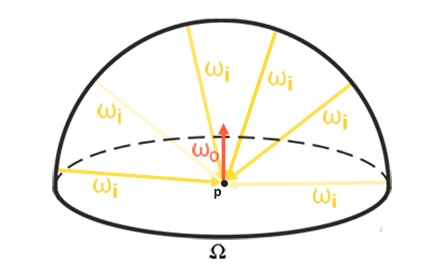
\includegraphics[scale=0.5]{hemisphere}}
    \caption{hemisphere}
  \end{figure}
  \singlespacing

La ecuaci\'on de render describe la radiancia de salida sobre un punto.
\begin{equation}
L_o(p, w_o) = \int_{\Omega} f_r(p, w_i, w_o)L_i(p, w_i)n\cdot{w_i}dw_i
\end{equation}
\singlespacing

Siendo $\Omega$ la hemiesfera centrada en el punto sobre la que calculamos la irradiancia,
$f_r$ representa el brdf, $Li$, la irradiancia de la escena, mientras que $n\cdot{w_i}$ toma en
cuenta el \'angulo entre la de incidencia de la luz sobre la superficie.

\begin{equation}
L_o(p, w_o) = \int_{\Omega} (k_d + \frac{c}{\pi} + 
k_s \frac{DFG}{4(w_o\cdot{n})(w_i\cdot{n})})L_i(p, w_i)n\cdot{w_i}dw_i
\end{equation}
\singlespacing

Los terminos $k_s$ y $k_d$ de la ecuacion de reflectancia son independientes, por lo que, de la
misma forma que en la iluminacion directa, los componentes se pueden separar en difuso y
especular.

\begin{equation}
L_o(p, w_o) = \int_{\Omega}
(k_d \frac{c}{\pi}) L_i(p, w_i)n\cdot{w_i}dw_i +
\int_{\Omega} 
k_s \frac{DFG}{4(w_o\cdot{n})(w_i\cdot{n})})L_i(p, w_i)n\cdot{w_i}dw_i
\end{equation}
\singlespacing

    \subsection{Componente difusa}
    La soluci\'on de la integral de la irradiancia de salida sobre $\Omega$ requiere samplear el entorno
    en todas las direcciones posibles. Es por ello que en tiempo real, la soluci\'on consiste en
    precomputar este c\'alculo.\\

    Habiendo separado la ecuaci\'on para la componente difusa y especular, podemos observar que el t\'ermino del difuso
    de Lambert es constante y lo podemos sacar de la integral.

    \begin{equation}
    L_o(p, w_o) = \int_{\Omega}
    (k_d \frac{c}{\pi}) L_i(p, w_i)n\cdot{w_i}dw_i=
    k_d \frac{c}{\pi} \int_{\Omega}
    (L_i(p, w_i)n\cdot{w_i}dw_i
    \end{equation}
    \singlespacing

        \subsubsection{Mapas de irradiancia}
        T\'ecnica IBL (\textit{Image Based Lighting}), que permite precalcular la irradiacia del entorno, utilizando una im\'agen
        de referencia y almacenarla en una nueva textura, el mapa de irradiancia. Para ello se 
        \todo[inline]{t\'enica IBL}
        \todo[inline]{
            Convolution is applying some computation to each entry in a data set considering all other entries in the data set;
            the data set being the scene's radiance or environment map. Thus for every sample direction in the cubemap, we take
            all other sample directions over the hemisphere $\Omega$ into account.
            To convolute an environment map we solve the integral for each output wo sample direction by discretely sampling a
            large number of directions wi over the hemisphere $\Omega$ and averaging their radiance. The hemisphere we build the sample
            directions wi from is oriented towards the output wo sample direction we're convoluting.
        }
        \todo[inline]{
            computed sum of all indirect diffuse light of the scene hitting some surface aligned along direction wo. Such a
            cubemap is known as an irradiance map seeing as the convoluted cubemap effectively allows us to directly sample the
            scene's (pre-computed) irradiance from any direction wo.
        }

        \begin{figure}[H]
            \vspace{0.5cm}
            \centering
            \frame{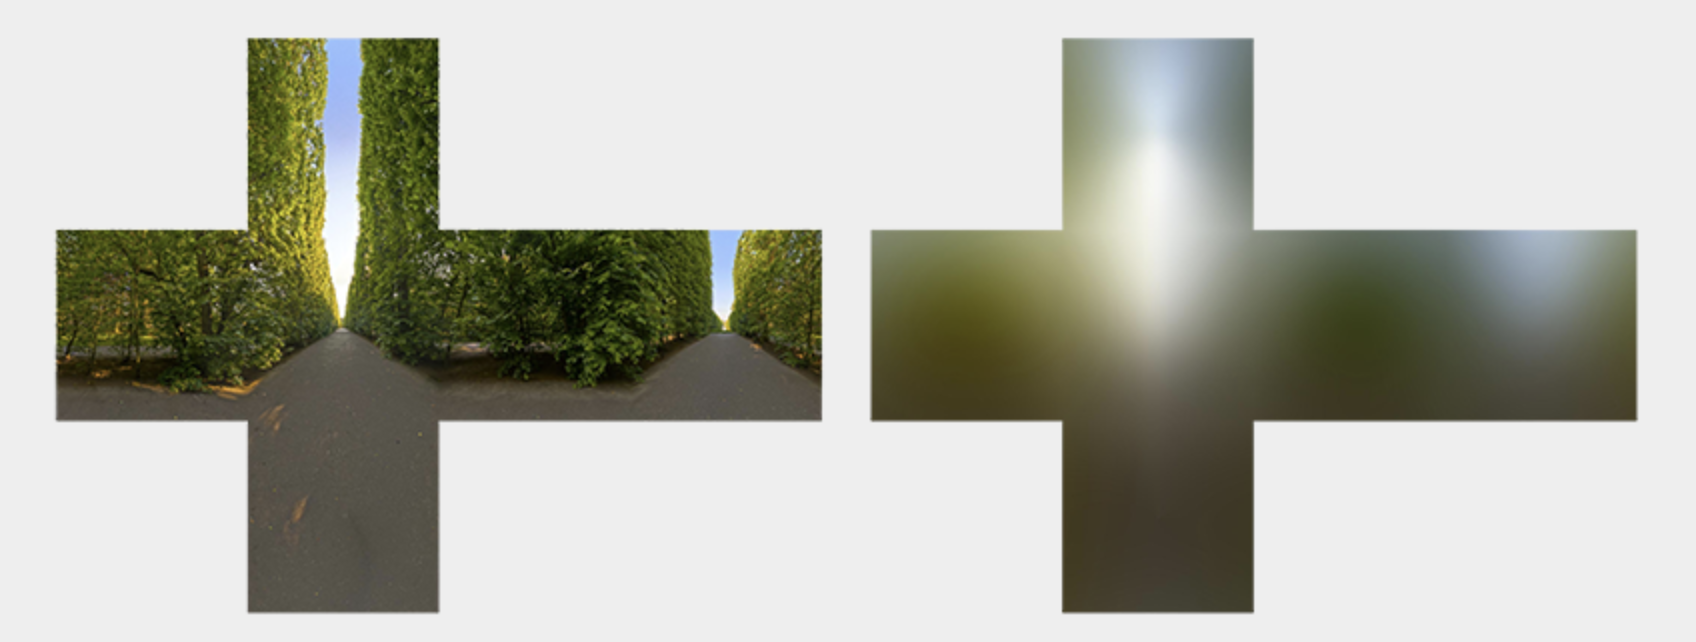
\includegraphics[scale=0.5]{irradiance_map}}
            \caption{Mapa de irradiancia como \textit{cubemap}}
        \end{figure}
        \singlespacing

        \subsubsection{Esf\'ericos harm\'onicos}
        \todo[inline]{
            \url{https://developer.nvidia.com/gpugems/gpugems2/part-ii-shading-lighting-and-shadows/chapter-10-real-time-computation-dynamic}
        }
    \subsection{Componente especular}

